\documentclass[aspectratio=169]{beamer}

\usetheme{Madrid}
\usecolortheme{default}
\setbeamertemplate{navigation symbols}{}

\usepackage[utf8]{inputenc}
\usepackage[T1]{fontenc}
\usepackage{lmodern}
\usepackage{amsmath}
\usepackage{booktabs}
\usepackage{array}
\usepackage{tabularx}
\usepackage{listings}
\usepackage{graphicx}
\usepackage{tikz}
\usetikzlibrary{arrows.meta,positioning,fit,shapes.geometric}
\usepackage{pgfplots}
\usepackage{pgf-pie}
\pgfplotsset{compat=1.18}
\graphicspath{{../images/}{images/}}

\setlength{\tabcolsep}{4pt}
\renewcommand{\arraystretch}{1.12}
\setlength{\columnsep}{0.035\textwidth}
\newcolumntype{L}[1]{>{\raggedright\arraybackslash}p{#1}}
\newcolumntype{Y}{>{\raggedright\arraybackslash}X}
\newcommand{\slidetablefont}{\scriptsize}
\lstset{basicstyle=\ttfamily\tiny,breaklines=true,columns=fullflexible}

\title{Item-Reviser Project Update}
\subtitle{Second Seminar Presentation: Orchestration, Prompting, and Evaluation}
\author{Abdul Samad}
\date{June 15, 2026}

\begin{document}

\begin{frame}
  \titlepage
\end{frame}

\begin{frame}{What I Worked On This Week}
  \begin{itemize}
    \item Implemented the full internal orchestration workflow for the item-reviser as an opt-in path.
    \item Moved prompt templates and prompt bindings into configuration so the system is easier to adapt.
    \item Generated a larger candidate benchmark, \texttt{candidate\_v1\_2000}, using a clustered agent-style authoring workflow.
    \item Ran two full 200-item evaluation experiments with the same local model:
    \begin{itemize}
      \item baseline pipeline with orchestration disabled
      \item orchestrated pipeline with routing, specialization, and validation enabled
    \end{itemize}
    \item Logged both experiments end-to-end in MLflow and compared their automatic metrics.
  \end{itemize}
\end{frame}

\begin{frame}{Implemented Orchestration Workflow}
  \centering
  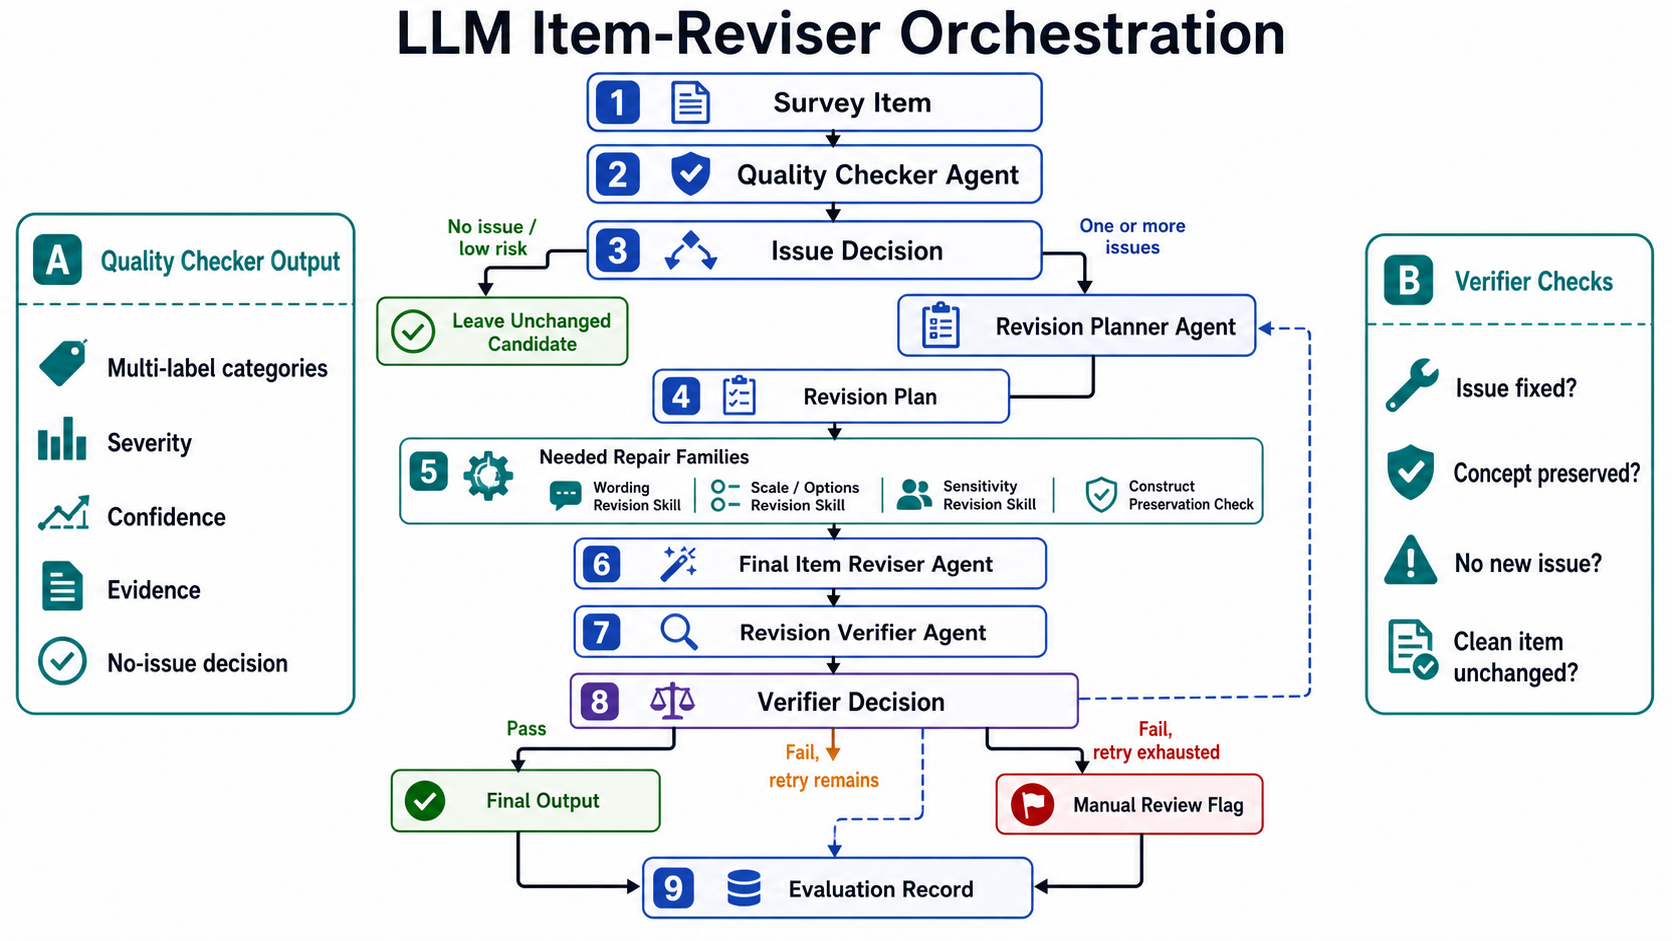
\includegraphics[width=0.84\textwidth,height=.84\textheight,keepaspectratio]{item_reviser_orchestration.png}

\end{frame}
\begin{frame}{Specialist Family Hierarchy}
  \scriptsize
  \centering
  \begin{tabularx}{0.96\textwidth}{L{0.28\textwidth}Y}
    \toprule
    Family & Routed taxonomy labels \\
    \midrule
    \textbf{Wording / clarity} &
    \texttt{leading\_question}, \texttt{loaded\_question}, \texttt{recall\_error}, \texttt{vague\_ambiguous}, \texttt{negative\_wording} \\
    \addlinespace[0.1cm]
    \textbf{Response options / scale} &
    \texttt{agree\_disagree\_scale}, \texttt{unbalanced\_scale}, \texttt{incomplete\_options}, \texttt{non\_exclusive\_options}, \texttt{missing\_scale\_labels}, \texttt{too\_many\_scale\_points}, \texttt{polarity\_mismatch} \\
    \addlinespace[0.1cm]
    \textbf{Construct alignment} &
    \texttt{double\_barreled} \\
    \addlinespace[0.1cm]
    \textbf{Bias / sensitivity} &
    \texttt{sensitive\_topic\_direct}, \texttt{social\_desirability} \\
    \addlinespace[0.1cm]
    \textbf{Questionnaire format} &
    \texttt{open\_closed\_mismatch} \\
    \bottomrule
  \end{tabularx}

  \vspace{0.16cm}

  \begin{alertblock}{Fallback rule}
    Low-confidence, mixed-family, unsupported, or conflicting cases go to the general fallback reviser.
  \end{alertblock}
\end{frame}
\begin{frame}{Prompting Method}
  \begin{columns}[T]
    \begin{column}{0.53\textwidth}
      \begin{block}{Design choices}
        \begin{itemize}
          \item Prompt templates live as Markdown files under \texttt{prompts/agents/}.
          \item Agent-to-prompt mapping, retry count, and timeouts are in \texttt{configs/prompt/default.yaml}.
          \item Every agent returns \textbf{strict JSON} against an explicit schema.
          \item Construct preservation and ``fix only what is supported'' are repeated across prompts.
          \item The router and validator are instructed \textbf{not} to rewrite the item.
        \end{itemize}
      \end{block}
    \end{column}
    \begin{column}{0.47\textwidth}
      \slidetablefont
      \begin{table}
        \centering
        \begin{tabularx}{\linewidth}{L{0.34\linewidth}Y}
          \toprule
          Agent & Main output \\
          \midrule
          Router & accept / revise / fallback + labels + confidence \\
          Planner & repair family + selected agent + instructions \\
          Specialist / fallback reviser & candidate revised item \\
          Validator & pass / retry / manual review \\
          \bottomrule
        \end{tabularx}
      \end{table}

      \vspace{0.2cm}

      \begin{alertblock}{Why this matters}
        The prompts are now modular enough that we can change routing policy or specialist behavior without editing core code.
      \end{alertblock}
    \end{column}
  \end{columns}
\end{frame}

\begin{frame}{Clustered Agent Workflow for \texttt{candidate\_v1\_2000}}
  \centering
  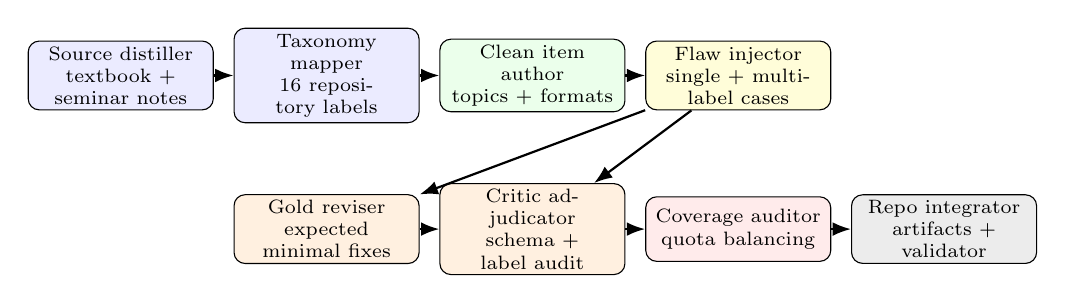
\begin{tikzpicture}[
    node distance=0.42cm and 0.25cm,
    every node/.style={font=\scriptsize},
    box/.style={
      draw,
      rounded corners,
      align=center,
      minimum width=2.35cm,
      text width=2.15cm,
      minimum height=0.82cm,
      inner sep=2pt
    },
    arrow/.style={-Latex, thick}
  ]
    \node[box, fill=blue!8] (a) {Source distiller\\textbook + seminar notes};
    \node[box, fill=blue!8, right=of a] (b) {Taxonomy mapper\\16 repository labels};
    \node[box, fill=green!8, right=of b] (c) {Clean item author\\topics + formats};
    \node[box, fill=yellow!15, right=of c] (d) {Flaw injector\\single + multi-label cases};

    \node[box, fill=orange!12, below=0.9cm of b] (e) {Gold reviser\\expected minimal fixes};
    \node[box, fill=orange!12, right=of e] (f) {Critic adjudicator\\schema + label audit};
    \node[box, fill=red!8, right=of f] (g) {Coverage auditor\\quota balancing};
    \node[box, fill=gray!15, right=of g] (h) {Repo integrator\\artifacts + validator};

    \draw[arrow] (a) -- (b);
    \draw[arrow] (b) -- (c);
    \draw[arrow] (c) -- (d);
    \draw[arrow] (d) -- (f);
    \draw[arrow] (d) -- (e);
    \draw[arrow] (e) -- (f);
    \draw[arrow] (f) -- (g);
    \draw[arrow] (g) -- (h);
  \end{tikzpicture}

  \vspace{0.18cm}

  \small
  \begin{itemize}
    \item Sources include the first six chapters of Saris and Gallhofer (2014) plus seminar materials and protocol notes.
    \item This is a \textbf{candidate} benchmark: reproducible and balanced, but still intended for manual review before any final claim.
  \end{itemize}
\end{frame}

\begin{frame}[shrink=4]{\texttt{candidate\_v1\_2000}: Benchmark Composition}
  \begin{columns}[T,onlytextwidth]
    \begin{column}{0.49\textwidth}
      \small
      \begin{itemize}
        \item Total rows: \textbf{2000}
        \item Clean controls: \textbf{400}
        \item Single-label flawed rows: \textbf{1280}
        \item Multi-label flawed rows: \textbf{320}
        \item All \textbf{16 taxonomy labels} appear exactly \textbf{120} times each.
        \item Difficulty is balanced across:
        \begin{itemize}
          \item 667 obvious
          \item 667 realistic
          \item 666 borderline
        \end{itemize}
      \end{itemize}

      \begin{block}{Coverage}
        14 topic areas and 9 response-format types are represented.
      \end{block}
    \end{column}
    \begin{column}{0.49\textwidth}
      \scriptsize
      \centering
      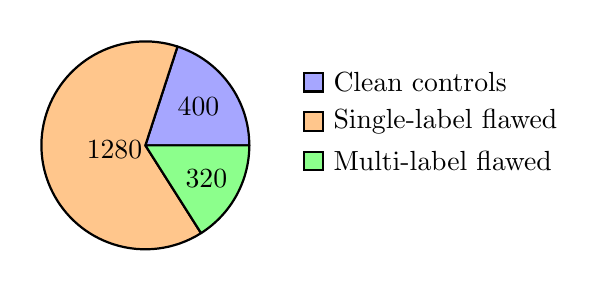
\begin{tikzpicture}
        \pie[
          text=legend,
          radius=1.32,
          sum=auto,
          color={blue!35, orange!45, green!45}
        ]{
          400/Clean controls,
          1280/Single-label flawed,
          320/Multi-label flawed
        }
      \end{tikzpicture}

      \vspace{0.08cm}

      \begin{alertblock}{Important caution}
        All 2{,}000 rows are marked \texttt{needs\_manual\_review: true}.
      \end{alertblock}
    \end{column}
  \end{columns}
\end{frame}

\begin{frame}[shrink=6]{Evaluation Metrics and Experiment Setup}
  \footnotesize
  \begin{columns}[T,onlytextwidth]
    \begin{column}{0.53\textwidth}
      \begin{block}{Automatic metrics}
        \begin{itemize}
          \item detection precision, recall, and F1
          \item exact-match rate on taxonomy output
          \item false-positive rate on clean items
          \item overcorrection rate on clean controls
          \item revision similarity metrics:
          \begin{itemize}
            \item exact revision match
            \item mean question similarity
            \item option Jaccard overlap
          \end{itemize}
        \end{itemize}
      \end{block}

      \begin{block}{Common setup}
        \begin{itemize}
          \item local \texttt{Qwen3.5-9B}
          \item same 200-item seed set
          \item same MLflow tracking setup
          \item 40 clean controls + 160 flawed items
        \end{itemize}
      \end{block}
    \end{column}
    \begin{column}{0.44\textwidth}
      \scriptsize
      \begin{table}
        \centering
        \begin{tabularx}{\linewidth}{L{0.31\linewidth}Y}
          \toprule
          Run & Condition \\
          \midrule
          Baseline\\(June 10, 2026) & Existing two-agent LLM path, orchestration disabled \\
          Orchestrated\\(June 11, 2026) & Router + planner + specialists/fallback + validator enabled \\
          \bottomrule
        \end{tabularx}
      \end{table}

      \vspace{0.06cm}

      \begin{alertblock}{Main comparison question}
        Does internal orchestration improve revision quality without increasing clean-item damage?
      \end{alertblock}
    \end{column}
  \end{columns}
\end{frame}

\begin{frame}{Results on the 200-Item Seed Set}
  \scriptsize
  \centering
  \begin{table}
    \begin{tabularx}{0.92\textwidth}{Yrrr}
      \toprule
      Metric & Baseline & Orchestrated & Delta \\
      \midrule
      Precision & 0.519 & \textbf{0.660} & +0.141 \\
      Recall & \textbf{0.847} & 0.816 & -0.032 \\
      F1 & 0.644 & \textbf{0.729} & +0.085 \\
      Exact match & 0.530 & \textbf{0.630} & +0.100 \\
      False positive rate on clean items & 0.000 & 0.000 & 0.000 \\
      Overcorrection rate & 0.375 & \textbf{0.000} & -0.375 \\
      Exact revision match rate & 0.125 & \textbf{0.200} & +0.075 \\
      Mean question similarity & 0.653 & \textbf{0.663} & +0.010 \\
      Mean option Jaccard & 0.267 & \textbf{0.299} & +0.032 \\
      Clean items changed & 15 / 40 & \textbf{0 / 40} & -15 \\
      \bottomrule
    \end{tabularx}
  \end{table}

  \vspace{0.12cm}

  \begin{block}{Headline}
    The orchestrated system improved overall balance: higher precision, higher F1, better exact match, and no clean-item overcorrection, at the cost of a small recall drop.
  \end{block}
\end{frame}

\begin{frame}{What the Orchestrated Run Actually Did}
  \begin{columns}[T,onlytextwidth]
    \begin{column}{0.52\textwidth}
      \slidetablefont
      \begin{table}
        \centering
        \begin{tabular}{lr}
          \toprule
          Trace summary & Count \\
          \midrule
          Router accept & 51 \\
          Router revise & 147 \\
          Router fallback & 2 \\
          Executed specialist route & 63 \\
          Executed fallback route & 86 \\
          Final revised outputs & 142 \\
          Final accepted outputs & 51 \\
          Final manual-review outputs & 7 \\
          Mean retry count & 0.06 \\
          \bottomrule
        \end{tabular}
      \end{table}
    \end{column}
    \begin{column}{0.45\textwidth}
      \small
      \begin{block}{Selected specialists}
        \begin{itemize}
          \item response-options / scale: 40
          \item bias / sensitivity: 10
          \item wording / clarity: 9
          \item construct alignment: 4
        \end{itemize}
      \end{block}

      \begin{alertblock}{Interpretation}
        The current system is still conservative. Many items are sent through the fallback reviser, especially mixed or multi-label cases. That gives us a clear next target for improvement.
      \end{alertblock}
    \end{column}
  \end{columns}
\end{frame}

\begin{frame}{Main Takeaways}
  \begin{itemize}
    \item The accept gate fixed a real baseline problem: the old pipeline still revised some clean items even when no issue was detected.
    \item Internal orchestration already looks scientifically useful, because it improves safety and overall balance rather than only pushing one metric.
    \item The large candidate benchmark is ready for auditing and can support stronger future stress tests than the 200-item seed set alone.
    \item The main weakness now is routing conservatism for multi-label and mixed-family items.
  \end{itemize}

  \vspace{0.2cm}

  \begin{block}{Next steps}
    Audit a reviewed subset from \texttt{candidate\_v1\_2000}, strengthen multi-label orchestration, and then rerun the comparison on a more demanding holdout benchmark.
  \end{block}
\end{frame}
\appendix

\begin{frame}{Backup Slides}
  \centering
  \Large Prompt Templates and Structured Outputs

  \vspace{0.5cm}

  \normalsize
  These slides are for deeper discussion if the orchestration design or LLM control mechanism comes up during questions.
\end{frame}

\begin{frame}[fragile]{Backup: Router / Quality Checker}
  \begin{columns}[T]
    \begin{column}{0.49\textwidth}
      \begin{block}{Prompt skeleton}
\begin{lstlisting}
You are the router and quality-checker agent for survey questionnaire items.

Task:
Decide whether the item should be accepted unchanged, revised by a supported specialist, or sent to the general fallback reviser.

Allowed taxonomy categories:
${allowed_categories}

Allowed route decisions:
${allowed_routes}

Survey item:
- question: ${question}
- response_options: ${response_options}
- target_concept: ${target_concept}
- topic: ${topic}

Instructions:
1. Return accept only when the item is sound.
2. Return revise when one supported issue is clear.
3. Return fallback for low-confidence, ambiguous, mixed, unsupported, or unsafe cases.
4. Do not revise the item in this step.
\end{lstlisting}
      \end{block}
    \end{column}
    \begin{column}{0.49\textwidth}
      \begin{block}{Output template}
\begin{lstlisting}
{
  "decision": "accept | revise | fallback",
  "taxonomy_labels": ["leading_question"],
  "confidence": 0.91,
  "evidence": "Short evidence from the item.",
  "rationale": "Why this route was chosen.",
  "recommended_route": "wording_clarity"
}
\end{lstlisting}
      \end{block}

      \begin{alertblock}{Presentation point}
        The router is the accept/revise/fallback gate. It does not rewrite the item.
      \end{alertblock}
    \end{column}
  \end{columns}
\end{frame}

\begin{frame}[fragile]{Backup: Revision Planner}
  \begin{columns}[T]
    \begin{column}{0.49\textwidth}
      \begin{block}{Prompt skeleton}
\begin{lstlisting}
You are the revision planner for a survey-item orchestration pipeline.

Task:
Convert the router output into a focused repair plan. Do not rewrite the item.

Suggested repair family:
${suggested_repair_family}

Suggested agent:
${suggested_agent}

Original survey item:
- question: ${question}
- response_options: ${response_options}
- target_concept: ${target_concept}

Router output:
${router_decision}

Detected issues:
${detected_issues}

Instructions:
1. Select the suggested repair family unless unsafe.
2. Use fallback when labels conflict or construct preservation is unsafe.
3. Write concrete instructions for the reviser.
4. Do not introduce a rewrite here.
\end{lstlisting}
      \end{block}
    \end{column}
    \begin{column}{0.49\textwidth}
      \begin{block}{Output template}
\begin{lstlisting}
{
  "repair_family": "wording_clarity",
  "selected_agent": "wording_clarity",
  "instructions": [
    "Remove the leading phrase.",
    "Preserve the target concept.",
    "Keep response options balanced."
  ],
  "fallback_reason": null,
  "rationale": "Clear leading-question issue maps safely to wording clarity."
}
\end{lstlisting}
      \end{block}

      \begin{alertblock}{Presentation point}
        The planner is an LLM planning step constrained by deterministic config mappings.
      \end{alertblock}
    \end{column}
  \end{columns}
\end{frame}

\begin{frame}[fragile]{Backup: Candidate Revision}
  \begin{columns}[T]
    \begin{column}{0.49\textwidth}
      \begin{block}{Specialist / fallback prompt skeleton}
\begin{lstlisting}
You are the wording and clarity specialist for survey questionnaire items.

Task:
Apply the revision plan while preserving the target construct.

Original survey item:
- question: ${question}
- response_options: ${response_options}
- target_concept: ${target_concept}

Detected issues:
${detected_issues}

Router output:
${router_decision}

Revision plan:
${revision_plan}

Instructions:
1. Fix only the routed issue.
2. Preserve the measurement intent.
3. Do not introduce a new scale or format issue.
4. Return strict JSON only.
\end{lstlisting}
      \end{block}
    \end{column}
    \begin{column}{0.49\textwidth}
      \begin{block}{Candidate revision output}
\begin{lstlisting}
{
  "question": "To what extent do you support or oppose improving the university's online services?",
  "response_options": [
    "Strongly oppose",
    "Somewhat oppose",
    "Neither support nor oppose",
    "Somewhat support",
    "Strongly support"
  ],
  "revision_notes": [
    "Removed leading wording.",
    "Used a balanced support-oppose scale."
  ],
  "changed": true,
  "rationale": "The revision removes the agreement cue while preserving the target concept."
}
\end{lstlisting}
      \end{block}

      \begin{alertblock}{Presentation point}
        Candidate revision is not a separate agent. It is the proposed item produced by a specialist or fallback reviser.
      \end{alertblock}
    \end{column}
  \end{columns}
\end{frame}

\begin{frame}[fragile]{Backup: Validator / Critic}
  \begin{columns}[T]
    \begin{column}{0.49\textwidth}
      \begin{block}{Prompt skeleton}
\begin{lstlisting}
You are the validator and critic agent for a survey-item revision pipeline.

Task:
Judge whether the candidate should pass, be retried, or be flagged for manual review. Do not rewrite the item.

Validation criteria:
${validation_criteria}

Original survey item:
${question}

Detected issues:
${detected_issues}

Revision plan:
${revision_plan}

Candidate revision:
${candidate_revision}

Remaining retry budget:
${remaining_retry_budget}

Instructions:
1. Pass only if the candidate fixes the issue and preserves the construct.
2. Retry when focused instructions can plausibly fix it.
3. Use manual_review for unsafe or construct-drifting cases.
\end{lstlisting}
      \end{block}
    \end{column}
    \begin{column}{0.49\textwidth}
      \begin{block}{Output template}
\begin{lstlisting}
{
  "status": "pass | retry | manual_review | failed",
  "rationale": "Why this validation decision was made.",
  "retry_instructions": [
    "Make the response options more balanced."
  ],
  "preserves_construct": true,
  "fixes_detected_issue": true,
  "introduces_new_issue": false
}
\end{lstlisting}
      \end{block}

      \begin{alertblock}{Presentation point}
        The validator is an LLM critic. It checks the candidate but does not rewrite it directly.
      \end{alertblock}
    \end{column}
  \end{columns}
\end{frame}

\end{document}
